\documentclass{beamer}
\usetheme{Warsaw}

\usepackage{pgf, tikz}
\usetikzlibrary{shapes,backgrounds,calc,arrows}

\usepackage{listings}
\lstset{
	tabsize=4,
	morekeywords={for,int,forelem,whilelem,null,if,else,in}
}

\usepackage{algorithmicx}
\usepackage{algpseudocode}
\usepackage{algorithm}
\usepackage{caption}
\usepackage{hyperref}

\usepackage{mathtools}
\DeclarePairedDelimiter\ceil{\lceil}{\rceil}
\DeclarePairedDelimiter\floor{\lfloor}{\rfloor}

\title{Utilizing a tuple-based optimization framework\\
for graph algorithms}

\author{L.J. Peters \and Prof. Dr. H.A.G. Wijshoff \and Dr. K.F.D. Rietveld}

\institute{Leiden Institute for Advanced Computer Science}
% - Use the \inst command only if there are several affiliations.
% - Keep it simple, no one is interested in your street address.

\date{December 22nd, 2016}

\AtBeginSection[]
{
  \begin{frame}<beamer>{Outline}
    \tableofcontents[currentsection]
  \end{frame}
}

% Let's get started
\begin{document}

\begin{frame}
  \titlepage
\end{frame}

\begin{frame}{Outline}
  \tableofcontents
  % You might wish to add the option [pausesections]
\end{frame}

% Section and subsections will appear in the presentation overview
% and table of contents.
\section{Introduction}

\subsection{Max-flow}

\begin{frame}{Max-flow}
	\begin{itemize}
		\item Given graph $G(V, E)$ with $V$ a set of nodes and $E$ a set of edges $(u, v, c)$, origin, destination and capacity

		\item A (set of) source node(s) $s$ and a (set of) sink node(s) $t$

		\item What is the maximum capacity from $s$ to $t$?
	\end{itemize}
\end{frame}

\begin{frame}{Max-flow II}
	\begin{figure}[h]
\centering
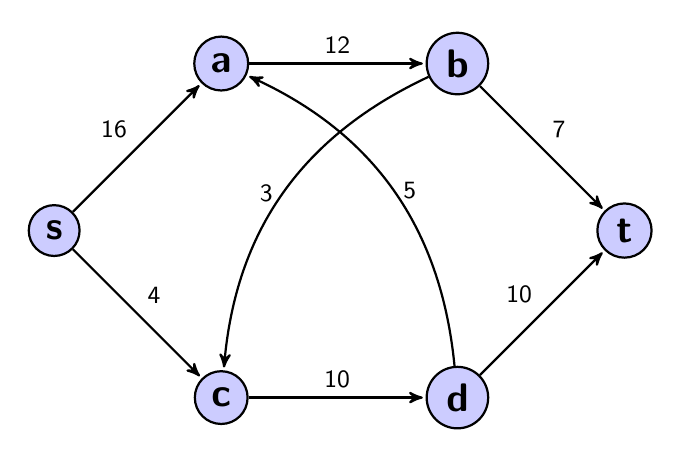
\begin{tikzpicture}[->,>=stealth',shorten >=1pt,auto,node distance=3cm,
  thick,main node/.style={circle,fill=blue!20,draw,font=\sffamily\Large\bfseries}]

  \node[main node] (1) {s};
  \node[main node] (2) [above right of=1] {a};
  \node[main node] (3) [right of=2] {b};
  \node[main node] (4) [below right of=1] {c};
  \node[main node] (5) [right of=4] {d};
  \node[main node] (6) [above right of=5] {t};

  \path[every node/.style={font=\sffamily\small}]
    (1) edge node {16} (2)
        edge node {4} (4)
    (2) edge node {12} (3)
    (3) edge [bend right] node [left] {3} (4)
        edge node {7} (6)
    (4) edge node {10} (5)
    (5) edge node {10} (6)
        edge [bend right] node [right] {5} (2)
    ;
\end{tikzpicture}
\caption{A simple graph with capacities}
\end{figure}
\end{frame}

\begin{frame}{Max-flow III}
	\begin{figure}[h]
\centering
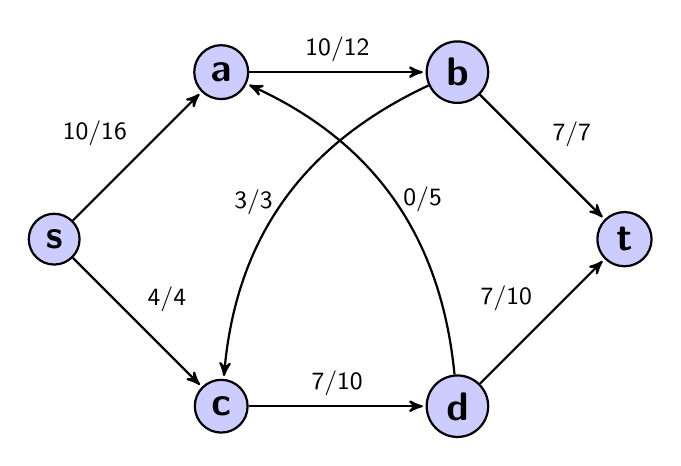
\begin{tikzpicture}[->,>=stealth',shorten >=1pt,auto,node distance=3cm,
  thick,main node/.style={circle,fill=blue!20,draw,font=\sffamily\Large\bfseries}]

  \node[main node] (1) {s};
  \node[main node] (2) [above right of=1] {a};
  \node[main node] (3) [right of=2] {b};
  \node[main node] (4) [below right of=1] {c};
  \node[main node] (5) [right of=4] {d};
  \node[main node] (6) [above right of=5] {t};

  \path[every node/.style={font=\sffamily\small}]
    (1) edge node {10/16} (2)
        edge node {4/4} (4)
    (2) edge node {10/12} (3)
    (3) edge [bend right] node [left] {3/3} (4)
        edge node {7/7} (6)
    (4) edge node {7/10} (5)
    (5) edge node {7/10} (6)
        edge [bend right] node [right] {0/5} (2)
    ;
\end{tikzpicture}
\caption{The max-flow solution to the previous graph}
\end{figure}
\end{frame}

\begin{frame}{Max-flow IV}
	Solutions available:
	\begin{description}
		\item[Augmenting path] Iteratively find paths with spare capacity to the final node
		\item[Push-Relabel] Create an excess flow at the source, and attempt to push that excess through the network
	\end{description}
\end{frame}

\subsection{forelem}

\begin{frame}{forelem}
	\begin{itemize}
		\item An abstraction language based on tuples
		\item Tranformations on the tuple form allow multiple implementations
			\begin{itemize}
				\item Loop dependent materialization
				\item Structure splitting
				\item Iteration space reduction.
			\end{itemize}
	\end{itemize}
\end{frame}

\begin{frame}[fragile]
	\begin{example}
		Sparse matrix-vector multiplication in forelem:
\begin{lstlisting}[mathescape]
for (i = N; i $\geq$ 1; i--)
{
    int sum = 0;
    forelem (j; j $\in$ pA.row[i])
        sum += B[A[j].col] * A[j].value;

    C[i] = sum;
}
\end{lstlisting}
	\end{example}
\end{frame}

\begin{frame}{forelem II}
	\begin{itemize}
		\item This is not executable code
		\item Need to create some index on the row number\pause
		\item Multidimensional array is possible, but wasteful
		\item Possible solutions:
			\begin{itemize}
				\item Sparse maps
				\item Nested arrays
				\item Index arrays
				\item \textellipsis more
			\end{itemize}
	\end{itemize}
\end{frame}

\section{Implementation}

\subsection{Push-Lift}

\begin{frame}{Push-Lift}
	Given graph $G(V, E)$ as before
	\begin{enumerate}
		\item Initialize height function $H(v)$ for $v \in V$:
			$$
			H(v) \gets \begin{cases}
				|V| & \text{if } v \text{ is a source} \\
				0 & \text{otherwise}
			\end{cases}
			$$

		\item Create preflow
		\item While there is a node with excess flow
			\begin{itemize}
				\item If a push is allowed, push
				\item Otherwise, lift
			\end{itemize}

		\item The max-flow is the current excess flow at the sink(s)
	\end{enumerate}
\end{frame}

\begin{frame}{Push-Lift}
	Push $(u, v, c)$ is legal iff
	\begin{itemize}
		\item There exists $e \in E: e(u, v, r) \land r \geq c$
		\item $H(u) = H(v) + 1$
	\end{itemize}

	Lift increases $H(u)$ such that at least one push is legal.

	Source and sink nodes are never considered.
\end{frame}

\subsection{DAS-4}

\begin{frame}{DAS-4}
	\begin{itemize}
		\item Parallel computer cluster
		\item Data sharing by message passing
		\item Need to adapt algorithm for this
	\end{itemize}
\end{frame}

\begin{frame}{Data distribution}
	\begin{itemize}
		\item Data distributed per node, using modulo
		\item Communication is expensive, so data sharing only as-needed\pause
			\begin{itemize}
				\item Node height known only to owner and neighbours
				\item Node excess known only to owner
			\end{itemize}\pause
		\item Because node excess is unknown, termination algorithm needed
			\begin{itemize}
				\item Safra's algorithm
			\end{itemize}
	\end{itemize}
\end{frame}

\begin{frame}{Safra's algorithm}
	\begin{itemize}
		\item Workers pass a white/black token with a counter
		\item When token arrives at first node without activity indication, work has finished
		\item Token passed only by inactive nodes, little overhead
		\item Token passed at most twice through all workers after work has finished
	\end{itemize}
\end{frame}

\subsection{Implementations}

\begin{frame}{Implememtations}
	\begin{itemize}
		\item Manually created from forelem specification
		\item Similar to adjacency lists
		\item Three implementations created for experiment:
			\begin{enumerate}
				\item Nested arrays
				\item Sparse arrays based on binary trees
				\item No materialization, checking validity while iterating
			\end{enumerate}\pause

		\item Third implementaiton intended as baseline, but was too slow to test.
	\end{itemize}
\end{frame}

\section{Experiments}

\subsection{Data sets}

\begin{frame}{Data sets}
	\begin{itemize}
		\item Real-world graphs from UFL spare matrix collection
			\begin{itemize}
				\item Biological network of DNA electrophoresis \texttt{vanHeukelem/cage11}
				\item Internet router topology \texttt{Pajek/Internet}
			\end{itemize}

		\item Synthetic graphs created by GTGraph
			\begin{itemize}
				\item Power law confirming networks generated by R-MAT
				\item Locally clustered networks generated by SSCA2
			\end{itemize}

		\item Source/sink selected for algorithm runtime
	\end{itemize}
\end{frame}

\begin{frame}
\begin{table}
	\centering

	\begin{tabular}{l | l | l | l | l}
		Name & Nodes & Edges & Source & Sink \\
		\hline
		cage11 & 39082 & 559722 & 1361 & 28129 \\
		internet & 124651 & 207214 & 94268 & 1046 \\
		rmat& 30000 & 5000000 & 89872 & 59366 \\
		ssca2 & 32768 & 1570139 & 21264 & 7066 \\
	\end{tabular}
	\caption{An overview of the data sets and configurations used.}
\end{table}
\end{frame}

\begin{frame}{Experiment}
	The experiment:
	\begin{itemize}
		\item Run each data set with different number of nodes
		\item Measure excecution time and initialization time
	\end{itemize}
\end{frame}

\subsection{Results}
\begin{frame}{Initialization time}
	\begin{figure}
		\includegraphics[width=0.6\textwidth]{graphs/graph_initialization}
		\caption{Cost of initialization as a function of the number of workers}
		\label{fig:initialization_time}
	\end{figure}
\end{frame}

\begin{frame}{Speed up}
	\begin{figure}
		\includegraphics[width=0.6\textwidth]{graphs/graph_speedup}
		\caption{Relative speed up when running a specific route on the datasets.}
		\label{fig:speedup_cage11}
\end{figure}
\end{frame}

\begin{frame}{Average runtime}
	\begin{figure}[b!]
		\centering
		\includegraphics[width=0.5\textwidth]{graphs/graph_implementations}
		\caption{Comparison of implementations by execution time on the \texttt{internet} data set.}
		\label{fig:implmementations}
	\end{figure}
\end{frame}

\section{Conclusion}

\begin{frame}
	\begin{itemize}
		\item Created 2 functional implementaitons of parallel Push-Lift using forelem
		\item Parallelism is very limited
			\begin{itemize}
				\item Very little locality in the algorithm
			\end{itemize}

		\item Overhead of message-passing data sharing is too expensive
	\end{itemize}
\end{frame}

\subsection{Future work}

\begin{frame}{Future work}
	\begin{itemize}
		\item Improve locality by improving data distribution
			\begin{itemize}
				\item Make use of local clustering in network
			\end{itemize}
		\item Improve message passing efficiency
			\begin{itemize}
				\item Send pushes and lifts in batches rather than individually
				\item Use asynchronous methods to avoid waiting in MPI
			\end{itemize}
		\item Automate implemenation derivation
			\begin{itemize}
				\item Include more of the materializations and transformations
				\item Combine transformations
			\end{itemize}
	\end{itemize}
\end{frame}

\appendix
\begin{frame}
	\Huge Any questions?
\end{frame}

\end{document}
